\section*{Модели экономического равновесия}
\addcontentsline{toc}{section}{Модели экономического равновесия}
\subsection*{Модель Вальраса-Маршалла}
\addcontentsline{toc}{subsection}{Модель Вальраса-Маршалла}

\textbf{Задание:}\\
Провести численный анализ моделей Вальраса-Маршалла первого и второго порядков в среде AnyLogic.\\

\textbf{Решение:}\\
\textit{Динамическая модель поведения рынка первого порядка по Вальрасу-Маршаллу}\\

$Q(t)$ -- объём продаж в текущий момент времени $t$\\
$P(t)$ -- рыночная цена товара\\
$Q^D(t) = a - b P(t)$ -- спрос на товар\\
$Q^S(t) = c + g P(t - \tau)$ -- предложение товара\\
$P^D(t) = A - BQ(t)$ -- цена спроса\\
$P^S(t) = C + GQ(t)$ -- цена предложения\\
$\tau$ -- задержка во времени, связанная с тем, что для производства товара и доставки его на рынок требуется некоторое время\\
$h, k > 0$ -- настраиваемые параметры модели

\begin{align*}
	\begin{cases}
		\dfrac{dP(t)}{dt} = h \left( Q^D(P(t)) - Q^S(P(t - \tau)) \right)\\[10pt]
		\dfrac{dQ(t)}{dt} = k \left( P^D(Q(t)) - P^S(Q(t)) \right)\\
	\end{cases}
\end{align*}

В соответствии с формулами, данная модель была реализована в среде моделирования AnyLogic. (Рисунок \ref{fig:warshall1})
\begin{figure}[h]
	\centering 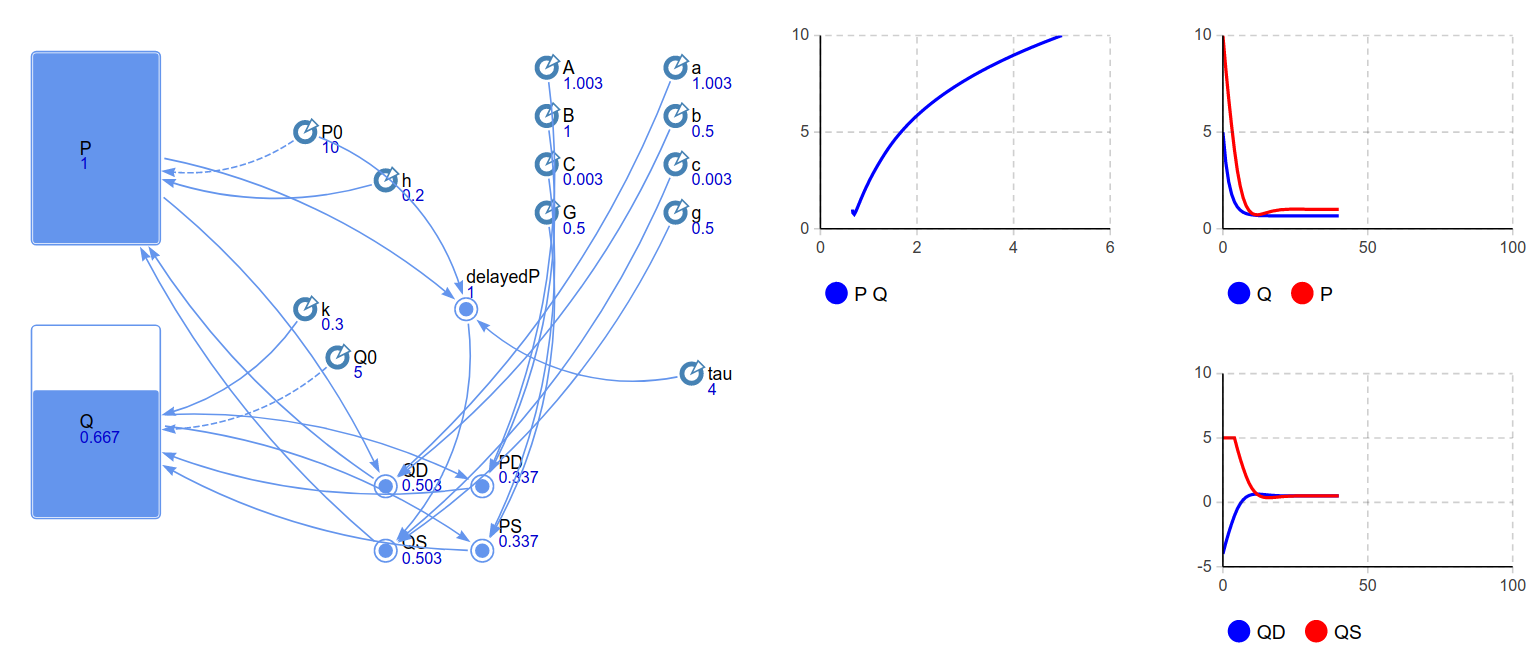
\includegraphics[scale=0.24]{warshall1}
	\caption{Результаты построения модели Вальраса-Маршалла первого порядка в AnyLogic}
	\label{fig:warshall1}
\end{figure}

\newpage

Симуляция показала, что спустя время модель придёт к состоянию равновесия -- устойчивый узел, независимо от того, какими были заданы входные параметры.\\

\textit{Динамическая модель поведения рынка второго порядка по Вальрасу-Маршаллу}\\

$Q(t)$ -- объём продаж в текущий момент времени $t$\\
$P(t)$ -- рыночная цена товара\\
$P^*$ -- равновесное значение цены\\
$Q^*$ -- равновесное значение объёма продаж\\
$a, b, q, r > 0$ -- настраиваемые параметры модели

\begin{align*}
	\begin{cases}
		\dfrac{dP(t)}{dt} = -a (P(t) - P^*) - q(Q(t) - Q^*)\\[10pt]
		\dfrac{dQ(t)}{dt} = -b (Q(t) - Q^*) + r(P(t) - P^*)\\
	\end{cases}
\end{align*}

В соответствии с формулами, данная модель была реализована в среде моделирования AnyLogic. (Рисунок \ref{fig:warshall2})
\begin{figure}[h]
	\centering 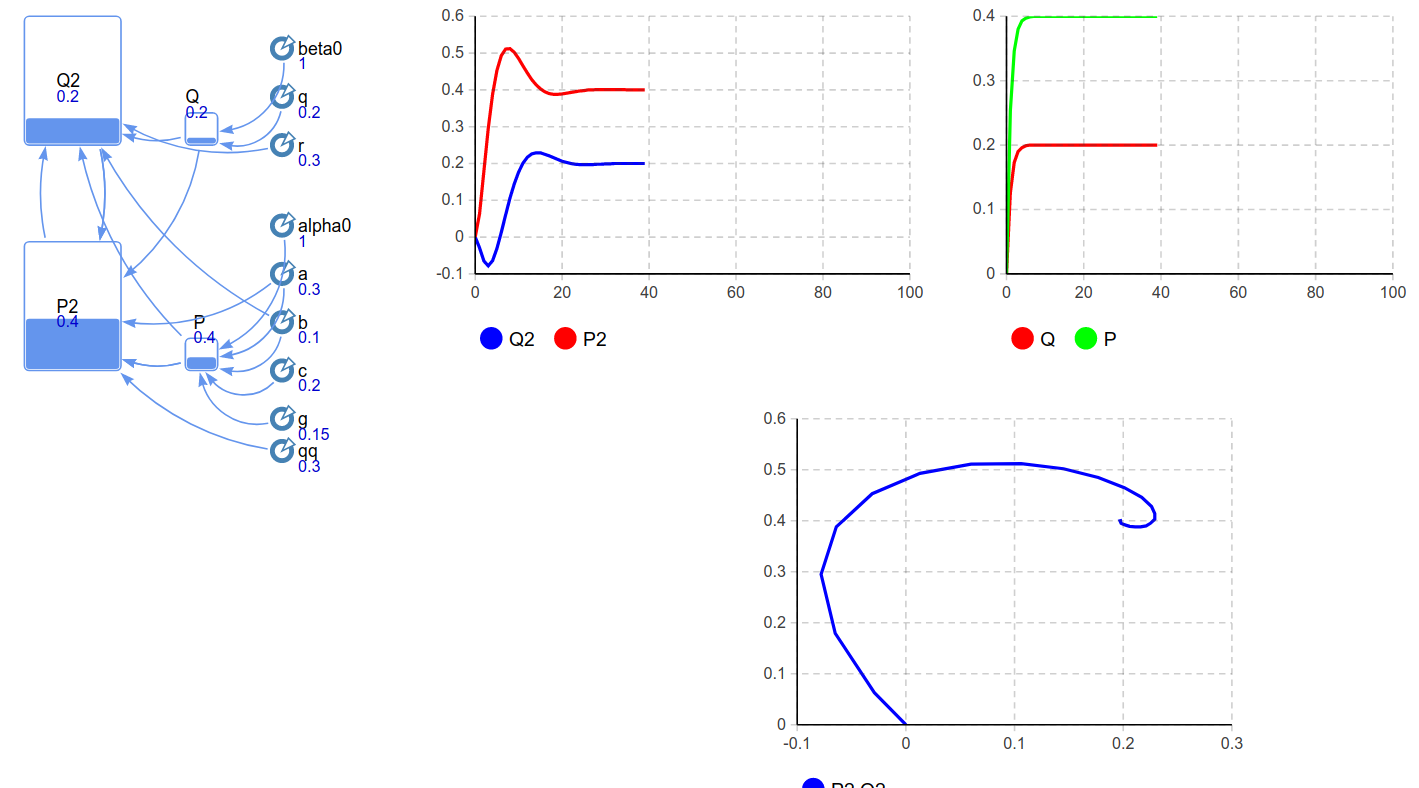
\includegraphics[scale=0.24]{warshall2}
	\caption{Результаты построения модели Вальраса-Маршалла второго порядка в AnyLogic}
	\label{fig:warshall2}
\end{figure}

Симуляция показала, что спустя время модель придёт к состоянию равновесия -- устойчивый фокус, независимо от того, какими были заданы входные параметры.\\

Таким образом, был проведен численный анализ модели Вальраса-Маршалла.